\documentclass{article}
\usepackage{graphicx, amssymb}
\usepackage{amsmath}
\usepackage{amsfonts}
\usepackage{amsthm}
\usepackage{kotex}
\usepackage{bm}
\usepackage{hyperref}
\usepackage{xcolor}
\usepackage{mathrsfs}
\usepackage{mathtools}
\usepackage{physics}
\usepackage{tikz}
\usetikzlibrary{decorations.markings}

\textwidth 6.5 truein 
\oddsidemargin 0 truein 
\evensidemargin -0.50 truein 
\topmargin -.5 truein 
\textheight 8.5in

\DeclareMathOperator{\cc}{\mathbb{C}}
\DeclareMathOperator{\rr}{\mathbb{R}}
\DeclareMathOperator{\bA}{\mathbb{A}}
\DeclareMathOperator{\fra}{\mathfrak{a}}
\DeclareMathOperator{\frb}{\mathfrak{b}}
\DeclareMathOperator{\frm}{\mathfrak{m}}
\DeclareMathOperator{\frp}{\mathfrak{p}}
\DeclareMathOperator{\slin}{\mathfrak{sl}}
\DeclareMathOperator{\Lie}{\mathsf{Lie}}
\DeclareMathOperator{\Alg}{\mathsf{Alg}}
\DeclareMathOperator{\Spec}{\mathrm{Spec}}
\DeclareMathOperator{\End}{\mathrm{End}}
\DeclareMathOperator{\rad}{\mathrm{rad}}
\newcommand*\Laplace{\mathop{}\!\mathbin\bigtriangleup}
\newcommand{\id}{\mathrm{id}}
\newcommand{\Hom}{\mathrm{Hom}}
\newcommand{\Sch}{\mathbf{Sch}}
\newcommand{\Ring}{\mathbf{Ring}}
\newcommand{\T}{\mathcal{T}}
\newcommand{\B}{\mathcal{B}}
\newcommand{\Mod}[1]{\ (\mathrm{mod}\ #1)}
\newtheorem{lemma}{Lemma}
\newtheorem{theorem}{Theorem}
\newtheorem{proposition}{Proposition}

\begin{document}


\title{Complex Analysis - Mid Term}
\author{SungBin Park, 20150462} 

\maketitle
Before starting, I'll prove Jordan's inequality, which will be used throughout this paper.
\begin{lemma}
For $R>0$,
\begin{equation*}
\int_0^\pi e^{-R\sin{\theta}}d\theta < \pi/R
\end{equation*}
\end{lemma}
\begin{proof}
Since $\sin{\theta}$ is a convex function in $0<\theta<\pi/2$, $\frac{2}{\pi}\theta\leq \sin{\theta}$ in $0\leq<\theta\leq \pi/2$. Therefore,
\begin{equation*}
\int_0^{\pi/2} e^{-R\sin{\theta}}d\theta \leq \int_0^{\pi/2} e^{-R\frac{2}{\pi}\theta}d\theta \leq \frac{\pi}{2R}\left(1-e^{-R}\right)<\frac{\pi}{2R}
\end{equation*}
Since $\int_0^\pi e^{-R\sin{\theta}}d\theta=2\int_0^{\pi/2} e^{-R\sin{\theta}}d\theta$,
\begin{equation*}
\int_0^\pi e^{-R\sin{\theta}}d\theta<\frac{\pi}{R}
\end{equation*}
\end{proof}
\section*{Problem 1}
Let's separate each term in the integral and calculate. I'll use the Fig. (\ref{Fig:P1}) as a contour in the integral. Since there is no singularity in the contour for all $R>1$, the integral is well defined for $R>1$.
\begin{figure}[h]
\centering
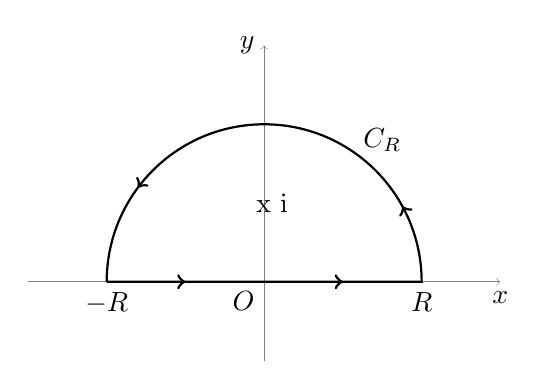
\begin{tikzpicture}[decoration={markings,
mark=at position 1cm with {\arrow[line width=1pt]{>}},
mark=at position 3cm with {\arrow[line width=1pt]{>}},
mark=at position 5cm with {\arrow[line width=1pt]{>}},
mark=at position 9cm with {\arrow[line width=1pt]{>}}
}
]
% The axes
\draw[help lines,->] (-3,0) -- (3,0) coordinate (xaxis);
\draw[help lines,->] (0,-1) -- (0,3) coordinate (yaxis);

% The path
\path[draw,line width=0.8pt,postaction=decorate] (-2,0) node[below] {$-R$} -- (2,0) node[below] {$R$} arc (0:180:2) ;

% The labels
\node[below] at (xaxis) {$x$};
\node[left] at (yaxis) {$y$};
\node[below left] {$O$};
\node at (1.5,1.8) {$C_{R}$};
\node at (0.1, 1) {x  i};
\end{tikzpicture}
\caption{The contour used in problem 1. x represent a pole of $\frac{1}{z^2+1}$ in the domain enclosed by contour.}
\label{Fig:P1}
\end{figure}

By Contour integral for fixed $R>1$,
\begin{equation}\label{Eq:P1-1}
\int_{-R}^R\frac{e^{ix}}{x^2+1}dx+\int_{C_R} \frac{e^{iz}}{z^2+1}dz=2\pi i \Res_{z=i} \left(\frac{e^{iz}}{z^2+1}\right)=\pi e^{-1}
\end{equation}
where $x$ is real valued variable. By the same way,
\begin{equation}\label{Eq:P1-2}
\int_{-R}^R \frac{xe^{ix}}{x^2+1}dx+\int_{C_R} \frac{ze^{iz}}{z^2+1}dz=2\pi i \Res_{z=i} \left(\frac{ze^{iz}}{z^2+1}\right)=i\pi e^{-1}.
\end{equation}
We know that
\begin{equation*}
\begin{split}
\text{Re}\int_{-R}^R\frac{e^{ix}}{x^2+1}dx&=\int_{-R}^R\text{Re}\frac{e^{ix}}{x^2+1}dx=\int_{-R}^R\frac{\cos(x)}{x^2+1}dx ~\text{ and } \\
\text{Im}\int_{-R}^R\frac{xe^{ix}}{x^2+1}dx&=\int_{-R}^R\text{Im}\frac{xe^{ix}}{x^2+1}dx=\int_{-R}^R\frac{x\sin(x)}{x^2+1}dx.
\end{split}
\end{equation*}
Therefore, if each $\int_{C_R}$ term in \eqref{Eq:P1-1} and \eqref{Eq:P1-2} converges to 0 as $R\rightarrow \infty$, we can get the desired result.

By the for remained term in \eqref{Eq:P1-1},
\begin{equation*}
\begin{split}
\lim\limits_{R\rightarrow \infty}\abs{\int_{C_R} \frac{e^{iz}}{z^2+1}dz}&=\abs{\int_0^\pi \frac{e^{iRe^{i\theta}}}{(R^2e^{i2\theta}+1)}Rie^{i\theta}d\theta}\leq \lim\limits_{R\rightarrow \infty} \int_0^\pi R\abs{\frac{e^{iRe^{i\theta}}}{(R^2e^{i2\theta}+1)}}d\theta \\
&\leq\lim\limits_{R\rightarrow \infty} \int_0^\pi R\abs{\frac{e^{-R\sin\theta}}{(R^2-1)}}d\theta\leq \lim\limits_{R\rightarrow \infty} \int_0^\pi R\abs{\frac{\pi/R}{(R^2-1)}}d\theta \text{ (Using Jordan's inequality)} \\
&=0.
\end{split}
\end{equation*}
By the same reason, $\lim\limits_{R\rightarrow \infty}\abs{\int_{C_R} \frac{ze^{iz}}{z^2+1}dz}=0$ since $z$ produce a $R$ term, making $\lim\limits_{R\rightarrow \infty}\abs{\int_{C_R} \frac{ze^{iz}}{z^2+1}dz}\leq \lim\limits_{R\rightarrow \infty}\abs{\int_0^\pi \frac{\pi R}{R^2-1}}d\theta=0$.

Therefore,
\begin{equation*}
\text{p.v.}\int_{-\infty}^\infty\frac{\cos(x)+x\sin(x)}{x^2+1}dx=\frac{2\pi}{e}
\end{equation*}

\section*{Problem 2}
I'll use the Fig. (\ref{Fig:P2}) as a contour in the integral.

\begin{figure}[h]
\centering
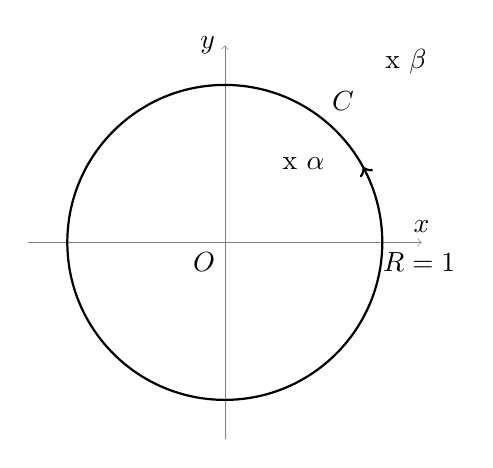
\begin{tikzpicture}[decoration={markings,
mark=at position 1cm with {\arrow[line width=1pt]{>}}
}
]
% The axes
\draw[help lines,->] (-2.5,0) -- (2.5,0) coordinate (xaxis);
\draw[help lines,->] (0,-2.5) -- (0,2.5) coordinate (yaxis);

% The path
\path[draw,line width=0.8pt,postaction=decorate] (2,0) node[below] {$~~~~~~~~R=1$} arc (0:360:2) ;

% The labels
\node[above] at (xaxis) {$x$};
\node[left] at (yaxis) {$y$};
\node[below left] {$O$};
\node at (1.5,1.8) {$C$};
\node at (1, 1) {x  $\alpha$};
\node at (2.3, 2.3) {x  $\beta$};
\end{tikzpicture}
\caption{The contour used in Problem 2. x represent poles and $\alpha$ and $\beta$ is some root of polynomial in the denominator.}
\label{Fig:P2}
\end{figure}
Recognizing $\sin\theta$ as $\frac{e^{i\theta}-e^{-i\theta}}{2i}$, we can rewrite the integral by
\begin{equation*}
\begin{split}
\int_0^{2\pi} \frac{1}{(1+2a\sin\theta+a^2)^2}d\theta&=\int_0^{2\pi} \frac{1}{\left(1+2a\left(\frac{e^{i\theta}-e^{-i\theta}}{2i}\right)+a^2\right)^2}d\theta\\
&=-\frac{1}{a^2i}\int_{C} \frac{z}{\left(z^2+\frac{i}{a}(1+a^2)z-1\right)^2}dz
\end{split}
\end{equation*}
where $z=e^{i\theta}$. Since $z^2+\frac{i}{a}(1+a^2)z-1=0$ has roots at $-i/a$ and $-ai$ and the $C$ is $S^1$ in $\mathbb{C}$, only $-ai$ is inside $C$. Therefore, 
\begin{equation*}
\int_{C} \frac{z}{\left(z^2+\frac{i}{a}(1+a^2)z-1\right)^2}dz=2\pi i\Res_{z=-ai}\frac{z}{\left(z^2+\frac{i}{a}(1+a^2)z-1\right)^2}=2\pi i\left(\frac{z}{(z+i/a)^2}\right)'\Bigg{|}_{z=-ia}=-\frac{2\pi i}{a^2}\frac{a^2+1}{(-a^2+1)^3}
\end{equation*}
Therefore,
\begin{equation*}
int_0^{2\pi} \frac{1}{(1+2a\sin\theta+a^2)^2}d\theta=\frac{2\pi(a^2+1)}{(-a^2+1)^3}.
\end{equation*}

\section*{Problem 3}
Using real analysis, we first reformulate the formula.
\begin{equation*}
\int_0^\infty \frac{\sin{x}}{x^{3/2}}dx=-\lim\limits_{x\rightarrow \infty} \frac{2\sin{x}}{x^{1/2}} + \lim\limits_{x\rightarrow 0+} \frac{2\sin{x}}{x^{1/2}} + 2\int_0^\infty \frac{\cos{x}}{x^{1/2}}dx=4\int_0^\infty \cos{t^2} dt
\end{equation*}
the last equality is derived by change $x$ by $t^2$. The limit is calculated by
\begin{equation*}
\begin{split}
&\lim\limits_{x\rightarrow \infty} \abs{\frac{2\sin{x}}{x^{1/2}}}\leq \lim\limits_{x\rightarrow \infty} \frac{2}{\abs{x^{1/2}}} = 0 \\
&\lim\limits_{x\rightarrow 0+} \frac{2\sin{x}}{x^{1/2}}=\lim\limits_{x\rightarrow 0+} \frac{2\sin{x}}{x}\frac{x}{x^{1/2}} = 1\cdot 0=0.
\end{split}
\end{equation*}

I'll evaluate $\int_0^\infty \cos{t^2} dt$. Consider a contour as in Fig. (\ref{Fig:P3}). There is no singularity of $e^{iz^2}$ in the region enclosed by the contour. Therefore,
\begin{equation*}
\int_0^R e^{ir^2} dr+ \int_R^0 e^{i(re^{i\pi/4})^2} e^{i\pi/4} dr + \int_0^{\pi/4} e^{iR^2e^{2\theta i}}Rie^{i\theta}d\theta = 0
\end{equation*}

Since $\int_0^{\pi/2}e^{{-R^2\sin(2\theta)}}\leq \frac{\pi}{2R^2}$ by Jordan's inequality, $\abs{\int_0^{\pi/4} e^{iR^2e^{2\theta i}}Rie^{i\theta}d\theta}\rightarrow 0$ as $R\rightarrow \infty$.
Also, $\int_R^0 e^{(re^{i\pi/4})^2} dr=\int_R^0 e^{i^2r^2} dr=-\int_0^R e^{-r^2} dr$ and the integral value goes to $-\sqrt{\pi}/2$ as $R\rightarrow \infty$. Therefore,
\begin{equation*}
\int_0^\infty e^{ir^2} dr=-e^{i\pi/4}\int_\infty^0 e^{i(re^{i\pi/4})^2} dr=e^{i\pi/4}\frac{\sqrt{\pi}}{2}
\end{equation*}
and $\int_0^\infty cos(x^2) dx = \text{Re}\int_0^\infty e^{ix^2} dx=\frac{1}{2}\sqrt{\frac{\pi}{2}}$.

Consequently,
\begin{equation*}
\int_0^\infty \frac{\sin{x}}{x^{3/2}}dx=\sqrt{2\pi}.
\end{equation*}

\begin{figure}[h]
\centering
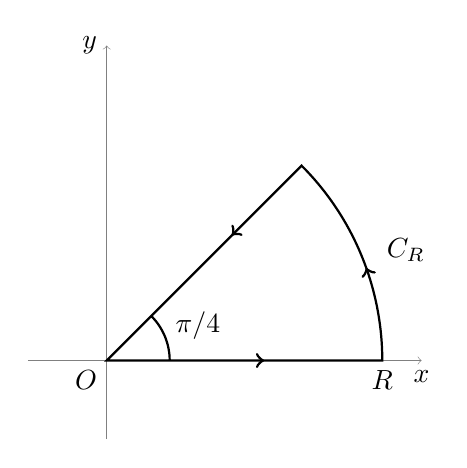
\begin{tikzpicture}[decoration={markings,
mark=at position 2cm with {\arrow[line width=1pt]{>}},
mark=at position 4.7cm with {\arrow[line width=1pt]{>}},
mark=at position 7.5cm with {\arrow[line width=1pt]{>}}
}
]
% The axes
\draw[help lines,->] (-1,0) -- (4,0) coordinate (xaxis);
\draw[help lines,->] (0,-1) -- (0,4) coordinate (yaxis);

% The path
\path[draw,line width=0.8pt,postaction=decorate] (0,0) -- (3.5,0) node[below] {$R$} arc (0:45:3.5) -- (0,0) -- (0.8,0) arc (0:45:0.8);

% The labels
\node[below] at (xaxis) {$x$};
\node[left] at (yaxis) {$y$};
\node[right] at (0.752, 0.448) {$\pi/4$};
\node[below left] {$O$};
\node at (3.8,1.4) {$C_{R}$};
\end{tikzpicture}
\caption{The contour used in problem 3. There is no pole of $e^{ir^2}$ in the domain enclosed by the contour.}
\label{Fig:P3}
\end{figure}
\end{document}
